\documentclass[a4paper]{article}

\usepackage[T2A]{fontenc}
\usepackage[utf8]{inputenc}
\usepackage[russian]{babel}


\usepackage{graphicx}
\usepackage{float}
\usepackage{mathtools}
\usepackage{wrapfig}
\usepackage{amsfonts, amssymb, amsmath, latexsym}
\usepackage{nicefrac}
\usepackage{hhline}
\usepackage{multirow}
\usepackage[colorinlistoftodos,bordercolor=orange,backgroundcolor=orange!20,linecolor=orange,textsize=scriptsize]{todonotes}
\usepackage[colorlinks=true,linkcolor=blue,citecolor=blue]{hyperref}       % hyperlinks
\usepackage{nicefrac}       % compact symbols for 1/2, etc.
\usepackage{nameref}
\usepackage{booktabs}       % professional-quality tables

\usepackage{algorithm}
\usepackage{algpseudocode}

\usepackage{xcolor, colortbl}
\usepackage{etoolbox}

% \graphicspath{ {./} }

\usepackage[verbose=true,letterpaper]{geometry}

\newgeometry{
    textheight=9in,
    textwidth=5.5in,
    top=1in,
    headheight=12pt,
    headsep=25pt,
    footskip=30pt
}

\usepackage{epigraph}

%

\newcommand{\argmin}{\mathop{\arg\!\min}}
\newcommand{\argmax}{\mathop{\arg\!\max}}

\newcommand{\Var}{\mathbb{V}}
\newcommand{\Exp}{\mathbb{E}}
\newcommand{\Cov}{\text{Cov}}
\newcommand{\makebold}[1]{\boldsymbol{#1}}
\newcommand{\mean}[1]{\overline{#1}}
\newcommand{\eps}{\varepsilon}
\renewcommand{\epsilon}{\varepsilon}

\newcommand{\partfrac}[2]{\frac{\partial #1}{\partial #2}}
\newcommand{\ttt}[1]{\texttt{#1}}
\newcommand{\term}[1]{\textbf{#1}}

\newcommand{\la}{\langle}
\newcommand{\ra}{\rangle}

\newcommand{\lp}{\left(}
\newcommand{\rp}{\right)}
\newcommand{\lf}{\left\{}
\newcommand{\rf}{\right\}}
\newcommand{\ls}{\left[}
\newcommand{\rs}{\right]}
\newcommand{\lv}{\left|}
\newcommand{\rv}{\right|}

\newcommand*{\affaddr}[1]{#1} % No op here. Customize it for different styles.
\newcommand*{\affmark}[1][*]{\textsuperscript{#1}}


\usepackage{amsthm}

\theoremstyle{definition}
\newtheorem{definition}{Определение}[section]

\newtheorem{exercise}{Задача}[section]

\newtheorem*{solution}{Решение}
\theoremstyle{remark}
\newtheorem*{remark}{Remark}

\makeatletter
\renewcommand{\l@section}{\@dottedtocline{1}{0em}{2.1em}}
\makeatother

% \setlength\epigraphwidth{.8\textwidth}
\setlength\epigraphrule{0pt}

\title{Работа 3.4.5 \\ Петля Гистерезиса}
\author{Шарапов Денис, Зелёный Николай, Б05-005}
\date{}

\usepackage{fancyhdr}
\pagestyle{fancy}
\fancyhf{}
\rhead{Работа 3.4.5}
\lhead{}
\cfoot{\thepage}
\usepackage{subcaption}
\usepackage[font={small}]{caption}

\begin{document}

    \maketitle
    \tableofcontents
    \newpage
    
\section{Аннотация}

\noindent \textbf{В работе используются:} автотрансформатор, понижающий трансформатор, интегрирующая ячейка, амперметр и вольтметр, резистор, делитель напряжения, электронный осциллограф, тороидальные образцы с двумя обмотками.
 
\section{Теоретические сведения}

К ферромагнетикам принадлежат железо, никель, кобальт, гадолиний, их многочисленные сплавы с другими металлами. К ним примыкают ферриты --- диэлектрики со структурой антиферромагнетика. \medskip

\noindent Магнитная индукция \textbf{$B$} и напряженность магнитного поля \textbf{$H$} в ферромагнитном материале неоднозначно связаны между собой: индукция зависит не только от напряженности, но и от предыстории образца.

\subsection{Экспериментальная установка}

\begin{figure}[h!]
    \centering
    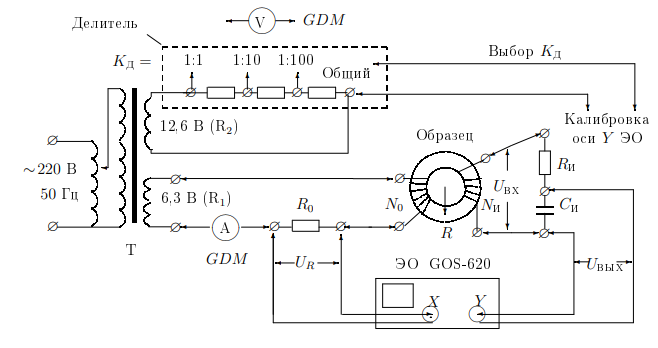
\includegraphics[width=\linewidth]{image/pic1.png}
    \caption{Схема установки}
\end{figure}

\noindent Схема установки приведена на рис. 1. Напряжение сети $(220 \mathrm{B}, 50$Гц$)$ через разделительный понижаюший трансформатор Тр подаётся на реостат $R_{1},$ ВКлючённый как потенциометр. Регулируемое напряжение $\sim 6,3$ В подведено к средним точкам переключателя $\mathrm{K}_{0}:$ в положении <<$\Pi$>> (петля) напряжение подводится к клеммам <<$6,3$>> на панели установки, В положении <<Д>> (делитель) --- к клеммам делителя напряжения. \medskip

\noindent С клемм <<$6,3$>> регулируемое напряжение подаётся на намагничивающуую обмотку~$N_{0}$ исследуемого образца. \medskip

\noindent Ток в обмотке $N_{0}$ измеряется мультиметром А. Напряжение с сопротивления $R_{0}$, включенного последовательно с обмоткой $N_{0}$, подаётся на вход $X$ электронного осциллографа (ЭО). Это напряжение пропорционально току в обмотке $N_{0}$, а следовательно и напряжённости $H$ магнитного поля в образце. \medskip

\noindent Для измерения магнитной индукции $B$ с измерительной обмотки $N_{\text {И }}$ на вход интегрируюшей $R C$ --- цепочки подаётся напряжение $U_{\mathrm{BX}},$ пропорциональное производной $\dot{B},$ a $\mathrm{c}$ выхода снимается напряжение $U_{\mathrm{BbIX}}=U_{C},$ пропорциональное величине $B,$ и подаётся на вход $Y$. \medskip

\noindent Замкнутая кривая, возникающая на экране, воспроизводит в некотором масштабе (различном для осей $X$ и $Y)$ петлю гистерезиса. Чтобы придать этой кривой количественный смысл, необходимо установить масштабы изображения, т.е. провести калибровку каналов $X$ и $Y$ ЭО. Для этого, во-первых, надо узнать, каким напряжениям (или токам) соответствуют амплитуды сигналов, видимых на экране, и во-вторых, --- каким значениям $B$ и $H$ соответствуют эти напряжения (или току). \medskip

\noindent Измерение напряжения с помошью осциллографа. Исследуемый сигнал подаётся на вход $X$ ЭО; длина $2 x$ горизонтальной черты, наблюдаемой на экране, характеризует удвоенную амплитуду сигнала. \medskip

\noindent Если известна чувствительность усилителя $K_{X}$ в вольтах на деление нгкалы экрана $(\mathrm{B} / \mathrm{\text{cм}}),$ то удвоенная амплитуда напряжения определяется произведением
$$
2 U_{X, 0}=2 x \cdot K_{X}
$$

\noindent Напряжение, подаваемое на ось $Y,$ измеряется аналогично. Калибровку осей осциллографа $\left(K_{X}\right.$ и $\left.K_{Y}\right)$ можно использовать для построения кривой гистерезиса в координатах $B$ и $H$. \medskip

\noindent Зная величину сопротивления $R_{0},$ с которого снимается сигнал, можно рассчитать чувствительность канала по току $K_{X I}=K_{X} / R_{0}[\mathrm{A} \;/$ дел $]$, затем определить цену деления шкалы ЭО в $A / M$
Проверка калибровки горизонтальной оси ЭО с помошью амперметра проводится при закороченной обмотке $N_{0} .$ Эта обмотка с помещённым В неё ферромагнитным образцом является нелинейным элементом, так что ток в ней не имеет синусоидальной формы, и это не позволяет связать амплитуду тока с показаниями амперметра. \medskip

\noindent При закороченной обмотке $N_{0}$ амперметр А измеряет эффективное значение синусоидального тока $I$эф , текущего через известное сопротивление $R_{0} .$ Сигнал с этого сопротивления подаётся на вход $X$ ЭО. Измерив $2 x$ длину горизонтальной прямой на экране, можно рассчитать $m_{X}$ --- чувствительность канала $X:$
$$
m_{X}=2 R_{0} \sqrt{2} I_{\ni \Phi} /(2 x) \quad[\mathrm{B} / \text { Дел}]
$$
Проверка калибровки вертикальной оси ЭО с помошью вольтметра. Сигнал с потенциометра $R_{1}$ подаётся на вход делителя напряжения $\left(\mathrm{K}_{0}\right.$ в положении "Д". Часть этого напряжения снимается с делителя с коэффициентом деления $K_{\text {Д }}(1 / 10$ или $1 / 100)$ и подаётся на вход $Y$ ЭО $($ вместо напряжения $\left.U_{C}\right) .$ Цифровой вольтметр $V$ измеряет напряжение $U_{\text {ЭФ }}$ на этих же клеммах делителя. Измерив $2 y$ --- длину вертикальной прямой на экране, можно рассчитать чувствительность канала $Y$:
$$
m_{Y}=2 \sqrt{2} U_{\ni \Phi} /(2 y) \quad[\mathrm{B} / \text { дел}]
$$

\section{Результаты измерений и обработка данных}

Параметры исследуемых образцов представлены в таблице 1.

\begin{table}[h!]
    \centering
    \caption{Параметры образцов}
    \begin{tabular}{|c|c|c|c|c|}
    \hline
                      & $N_0$, витков & $N_U$б витков & $S$, см$^2$ & $2\pi R$, см \\ \hline
    Феррит            & 45            & 400           & 3,0         & 25           \\ \hline
    Пермаллой         & 15            & 300           & 0,66        & 14,1         \\ \hline
    Кремнистое железо & 20            & 200           & 2           & 11           \\ \hline
    \end{tabular}
    \end{table}

\subsection{Каллибровка}

Откалибруем X канал осциллографа, измерив зависимость показаний осциллографа от тока через амперметр. Занесем результаты в таблицу 2. Рассчитаем коэффециент пересчета делений в ток $dI$ для всех диапазонов. \medskip

Откалибруем Y канал осциллографа, сравним показания вольтметра и осциллографа и занесем результаты в таблицу 3. Домножив $U$ на $2\sqrt{2}$ получим, что в среднем  $U_{V}$ отличается от $U_{O}$ на 2\%.

\begin{table}[h!]
    \centering
    \caption{Каллибровка канала X}
    \begin{tabular}{|cc|cc|cc|}
    \hline
    \multicolumn{2}{|c|}{$X = 20$ мВ}                & \multicolumn{2}{c|}{$X = 50$ мВ}                & \multicolumn{2}{c|}{$X = 100$ мВ}              \\ \hline
    \multicolumn{1}{|c|}{Дел}        & $I$, мА       & \multicolumn{1}{c|}{Дел}        & $I$, мА       & \multicolumn{1}{c|}{Дел}       & $I$, мА       \\ \hline
    \multicolumn{1}{|c|}{0}          & 6             & \multicolumn{1}{c|}{0}          & 6             & \multicolumn{1}{c|}{0}         & 6             \\ \hline
    \multicolumn{1}{|c|}{1}          & 34            & \multicolumn{1}{c|}{1}          & 89            & \multicolumn{1}{c|}{1}         & 176           \\ \hline
    \multicolumn{1}{|c|}{2}          & 70            & \multicolumn{1}{c|}{2}          & 173           & \multicolumn{1}{c|}{2}         & 351           \\ \hline
    \multicolumn{1}{|c|}{3}          & 106           & \multicolumn{1}{c|}{3}          & 266           & \multicolumn{1}{c|}{3}         & 536           \\ \hline
    \multicolumn{1}{|c|}{4}          & 143           & \multicolumn{1}{c|}{4}          & 354           & \multicolumn{1}{c|}{4}         & 707           \\ \hline
    \multicolumn{1}{|c|}{5}          & 181           & \multicolumn{1}{c|}{5}          & 442           & \multicolumn{1}{c|}{5}         & 896           \\ \hline
    \multicolumn{2}{|c|}{$dI \approx 36,0 \pm 3$ мА} & \multicolumn{2}{c|}{$dI \approx 88,4 \pm 3$ мА} & \multicolumn{2}{c|}{$dI \approx 180 \pm 6$ мА} \\ \hline
    \end{tabular}
    \end{table}

    \begin{table}[h!]
        \centering
        \caption{Каллибровка канала Y}
        \begin{tabular}{|c|c|}
        \hline
        $U_V$, мВ & $U_O$, мВ \\ \hline
        20    & 50    \\ \hline
        40    & 110   \\ \hline
        60    & 170   \\ \hline
        80    & 220   \\ \hline
        100   & 275   \\ \hline
        120   & 325   \\ \hline
        140   & 390   \\ \hline
        \end{tabular}
        \end{table}

\subsection{Исследование образцов}

Для каждого образца запишем значения коэффициентов усиления $K_{x}$ и $K_{y}$, ток $I_{\text{эф}}$. Измерим двойные амплитуды для коэрцитивной силы $2x(c)$ и индукции насыщения $2y(s)$. Результаты представлены в таблице 4.

\begin{table}[h!]
    \centering
    \caption{Результаты измерения коэффициентов усиления и двойных амплитуд образцов}
    \begin{tabular}{|c|c|c|c|c|c|}
    \hline
                      & $K_x$, $\frac{\text{мВ}}{\text{дел}}$ & $K_y$, $\frac{\text{мВ}}{\text{дел}}$ & $I_{\text{эф}}$, мА & $2x$, дел & $2y$, дел \\ \hline
    Феррит            & 100   & 20    & 990                 & 6,2       & 6,8       \\ \hline
    Пермаллой         & 20    & 50    & 218                 & 7         & 3,5       \\ \hline
    Кремнистое железо & 10    & 50    & 92,6                & 7,1       & 8         \\ \hline
    \end{tabular}
\end{table}
 	
Снимем для каждого образца начальную кривую намагничивания (табл. 5-7), плавно уменьшая ток до нуля и отмечая вершины частных петель.

\newpage
  	
  		\begin{table}[h!]
  		\caption{Начальная кривая намагничивания для кремнистого железа}
  		\begin{center}
  			\begin{tabular}{|c|c|c|c|c|c|c|c|c|c|c|c|c|c|} 
  				\hline 
  				№ &  1 &  2 & 3 & 4 & 5 &  6 &  7 & 8 & 9 & 10  &  11 &  12 & 13  \\ 	\hline
  				
  			 $ x $, дел & 2,0 & 1,8 & 1,6 & 1,5 & 1,4 & 1,2 & 1,0 & 0,8 & 0,6 & 0,5 & 0,4 & 0,2 & 0,0 \\
  				 $ y $, дел & 3,0 & 2,8 & 2,7 & 2,5 & 2,3 & 2,1 & 2,0 & 1,6 & 1,2 & 0,7 & 0,4 & 0,1 & 0,0 \\
  				\hline
  				
  			\end{tabular}
  		\end{center}
  	\end{table}

		\begin{table}[h!]
		\caption{Начальная кривая намагничивания для пермаллоя}
		\begin{center}
			\begin{tabular}{|c|c|c|c|c|c|c|c|c|c|c|c|c|c|} 
				\hline 
				№ &  1 &  2 & 3 & 4 & 5 &  6 &  7 & 8 & 9 & 10  &  11 &  12 &13   \\ 	\hline
				
			$ x $, дел & 3,0 & 2,8 & 2,6 & 2,4 & 2,2 & 2,0 & 1,8 & 1,5 & 1,2 & 0,8 & 0,5 & 0,2 & 0,0 \\
			 $ y $, дел & 1,8 & 1,7 & 1,5 & 1,4 & 1,1 & 1,0 & 0,9 & 0,7 & 0,5 & 0,4 & 0,2 & 0,1 & 0,0 \\
				\hline
				
			\end{tabular}
		\end{center}
	\end{table}

    \begin{table}[h!]
        \caption{Начальная кривая намагничивания для феррита}
        \begin{center}
            \begin{tabular}{|c|c|c|c|c|c|c|c|c|c|c|c|c|c|} 
                \hline 
                № &  1 &  2 & 3 & 4 & 5 &  6 &  7 & 8 & 9 & 10  &  11 &  12 &13   \\ 	\hline
                
            $ x $, дел &3,0 & 2,5 & 2,3 & 1,8 & 1,6 & 1,4 & 1,2 & 1,0 & 0,8 & 0,6 & 0,4 & 0,2 & 0,0 \\
             $ y $, дел & 3,6 & 3,4 & 3,3 & 3,1 & 3,0 & 2,7 & 2,4 & 2,2 & 2,0 & 1,2 & 0,5 & 0,2 & 0,0 \\
                \hline
                
            \end{tabular}
        \end{center}
    \end{table}

Восстановим предельные петли для образцов и рассчитаем $B$ и $H$. После чего рассчитаем коэрцитивную силу $H_{c}$ и индукцию насыщения $B_{s}$ для каждого образца. Результаты измерений внесём в таблицу 8.

\begin{table}[h!]
    \centering
    \caption{Результаты измерений магнитной индукции и напряженности для: 1. феррит; 2. пермаллой; 3. кремнистое железо}
    \begin{tabular}{|c|c|c|c|c|}
    \hline
      & $H$, A / м             & $B$, Тл / дел                            & $H_c$, A / м           & $B_s$, Тл / дел                            \\ \hline
    1 & $9,0 \pm 1,0$   & $(3,33 \pm 0,6) \cdot 10^{-2}$ & $8,1 \pm 0,2$  & $(12,9 \pm 0,02) \cdot 10^{-2}$ \\ \hline
    2 & $10,6 \pm 1,2$  & $1,01 \pm 0,2$                 & $24,4 \pm 0,5$ & $1,82 \pm 0,6$                  \\ \hline
    3 & $90,9 \pm 10,1$ & $0,20 \pm 0,03$                & $54,5 \pm 0,8$ & $0,70 \pm 0,1$                  \\ \hline
    \end{tabular}
    \end{table}

Из графиков, представленных на рисунках 2-4 определим максимальные значения дифференциальной магнитной проницаемости. Результаты внесём в таблицу 9.

\begin{table}[h!]
    \centering
    \caption{Результаты измерения максимальной магнитной проницаемости}
    \begin{tabular}{|c|c|}
    \hline
                      & $\mu_{max}$                \\ \hline
    Феррит            & $(7,6 \pm 0,6)\cdot 10^3$  \\ \hline
    Пермаллой         & $(89,7 \pm 7,6)\cdot 10^3$ \\ \hline
    Кремнистое железо & $(30,6 \pm 2,9)\cdot 10^3$ \\ \hline
    \end{tabular}
    \end{table}

    \begin{figure}[h!]
        \centering
        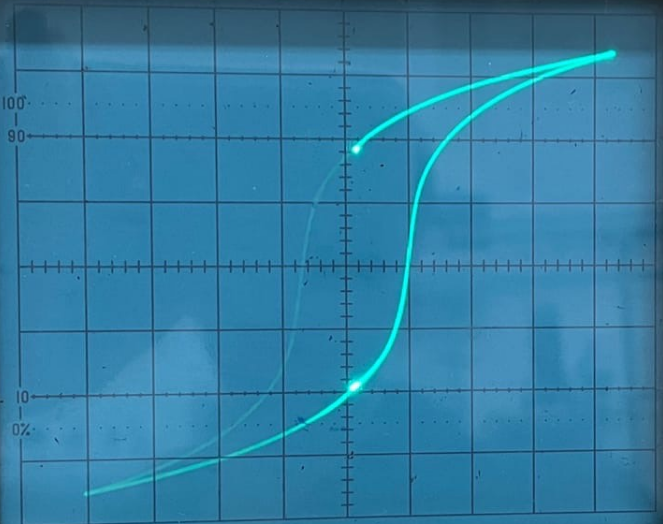
\includegraphics[width=0.5\linewidth]{image/ferrit.png}
        \caption{Петля Гистериза для феррита}
    \end{figure}

    \begin{figure}[h!]
        \centering
        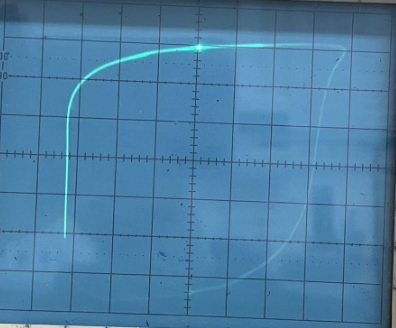
\includegraphics[width=0.5\linewidth]{image/perm.png}
        \caption{Петля Гистериза для пермаллоя}
    \end{figure}

    \begin{figure}[h!]
        \centering
        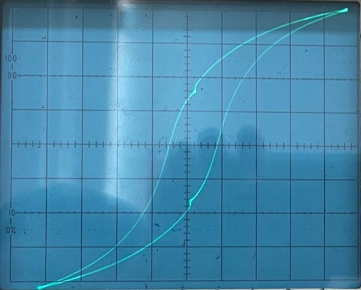
\includegraphics[width=0.5\linewidth]{image/krfer.png}
        \caption{Петля Гистериза для кремнистого железа}
    \end{figure}

    \section{Вывод}

    Петля гистерезиса является качественной характеристикой намагничивания ферромагнетика, показывающая такие эффекты, как домены, скачки Баркгаузена (которые можно было бы увидеть при значительно большем масштабе) и т.д.
    
\end{document}
